\documentclass[xcolor=dvipsnames]{beamer}
\usepackage[english]{babel}
\usepackage[latin1]{inputenc}
\usepackage{times}
\usepackage[T1]{fontenc}
\usepackage{graphicx}
\usepackage[absolute, overlay]{textpos}
\usepackage{tikz}
\usepackage{multimedia}
\usepackage{soul}
\usepackage{cancel}
\def\urltilda{\kern -.15em\lower .7ex\hbox{\~{}}\kern .04em}
\def\deg{^{\circ}}

\setlength{\TPHorizModule}{0.01\textwidth}
\setlength{\TPVertModule}{\TPHorizModule}
\definecolor{darkyellow}{rgb}{1,0.75,0}
\definecolor{black}{rgb}{0,0,0}
\definecolor{skyblue}{rgb}{0.7,0.8,1.0}
\definecolor{black}{rgb}{0,0,0}
\definecolor{darkgrey}{rgb}{0.3,0.3,0.3}
\definecolor{medgrey}{rgb}{0.5,0.5,0.5}
\definecolor{lightgrey}{rgb}{0.8,0.8,0.8}
\definecolor{lightMahogany}{rgb}{0.9,0.8,0.8}

\newcommand{\cblue}[1]{{\color[rgb]{0.1, 0.0, 0.6} #1}}
\newcommand{\cgreen}[1]{{\color[rgb]{0.0, 0.6, 0.1} #1}}
\newcommand{\corange}[1]{{\color[rgb]{0.9, 0.5, 0.0} #1}}
\newcommand{\cbluewhen}[2]{{\color#2[rgb]{0.1, 0.0, 0.6} #1}}
\newcommand{\cgreenwhen}[2]{{\color#2[rgb]{0.0, 0.6, 0.1} #1}}
\newcommand{\corangewhen}[2]{{\color#2[rgb]{0.9, 0.5, 0.0} #1}}

\newcommand{\manual}[1]{
  \begin{tikzpicture}[x=\textwidth, y=0.82\textheight]%, >=angle 90]
    \useasboundingbox (0, 0) rectangle (1, 1);
    #1
  \end{tikzpicture}
}

%%% Custom nodes.

\newcommand{\basenode}[4]{
  \node[outer sep=6pt, anchor=#3] (#1) at (#2){#4};
}

\newcommand{\emptynode}[2]{
  \basenode{#1}{#2}{base}{}

}

\newcommand{\minipagenode}[5]{
  \basenode{#1}{#2}{#3}{
    \begin{minipage}{#4}
      \vspace*{-12pt}
      {#5}
      \vspace*{-8pt}
  \end{minipage}}

}

\newcommand{\imagenode}[5]{
  \minipagenode{#1}{#2}{#3}{#4}{%
    \includegraphics[width=\textwidth]{#5}%
  }
}

%%% Connectors.

\newcommand{\connect}[4]{%
  \draw[<->, color=darkpurple, line width=1pt, out=#3, in=#4] (#1) to (#2);
}
\newcommand{\connectcolor}[5]{%
  \draw[<->, color=#5, line width=1pt, out=#3, in=#4] (#1) to (#2);
}
\newcommand{\hconnect}[3]{%
  \draw[<->, color=darkpurple, line width=1pt]
  (#1.east) .. controls +(right:#3) and +(left:#3) .. (#2.west);
}
\newcommand{\vconnect}[3]{%
  \draw[<->, color=darkpurple, line width=1pt]
  (#1.south) .. controls +(down:#3) and +(up:#3) .. (#2.north);
}

\newenvironment{litemize}
{\usebeamercolor[fg]{item color}%
\scriptsize\begin{list}{$\bullet$}{%
\setlength{\itemindent}{0pt}%
\setlength{\labelwidth}{10pt}%
\setlength{\leftmargin}{15pt}%
}}
{\end{list}}

\mode<presentation>
{
  \usetheme{Warsaw}
  \usecolortheme[named=Mahogany]{structure}	
  \setbeamercovered{transparent}
  \setbeamercolor*{section in toc}{bg=white, fg=Mahogany}
}

%\beamerdefaultoverlayspecification{<+->}

\AtBeginSubsection[]
{
  \begin{frame}<beamer>
    \frametitle{Outline}
  \begin{columns}[t]
	\column{0.8\textwidth}
	\tableofcontents[sections={1-3}, currentsection, currentsubsection]
  \end{columns}	
  \end{frame}
}

\setbeamertemplate{subsection in head/foot shaded}
{\textcolor{structure!70!white}{\insertsubsectionhead}}
\setbeamertemplate{subsection in head/foot}{\textcolor{white}\insertsubsectionhead}

\title[{\textcolor{white}The Astroparticle Road to New Physics}]{\textcolor{white}{The Astroparticle Road to New Physics}}
\author[\textcolor{medgrey}{Pat Scott -- Feb 19 -- STFC ERF Interview}]{Pat Scott}
\institute{\small{Department of Physics, McGill University}}
\date[Feb 19 2012]{February 19 2013}
\pgfdeclareimage[height=0.7cm]{university-logo}{McGill_crest}
\logo{\pgfuseimage{university-logo}}
\subject{Talks}

\begin{document}

\begin{frame}
  \titlepage
\end{frame}


\begin{frame}
\frametitle{Finding Beyond the Standard Model (BSM) Physics}

\begin{columns}

\column{0.57\textwidth}
A story of complementarity\ldots

\begin{itemize}
\item \footnotesize Existing data give us some constraints
\visible<3->{\item Direct searches for dark matter constrain cross-sections with nuclei}
\visible<4->{\item Accelerator searches rule out lighter masses}
\visible<5->{\item Indirect searches for dark matter constrain annihilation cross-sections (+ some nuclear cross-sections)}
\end{itemize}

\column{0.44\textwidth}
\raggedright
\only<1-2>{\visible<2>{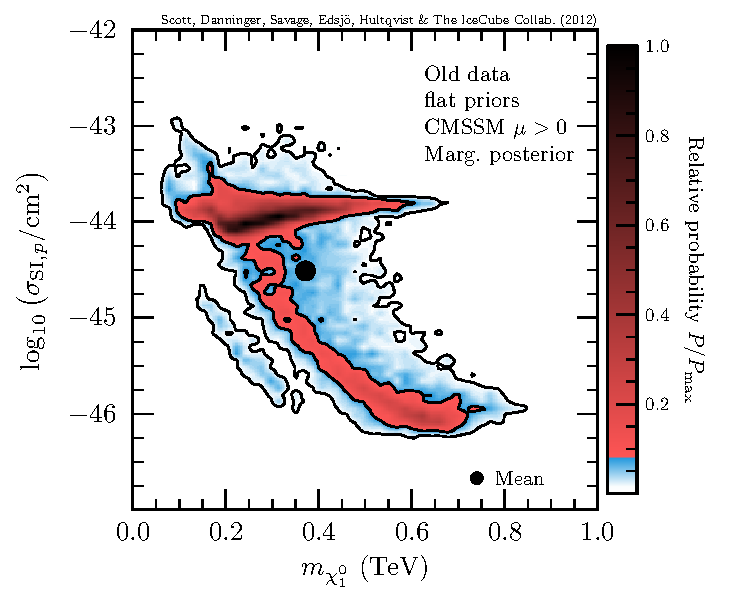
\includegraphics[height=0.95\linewidth, trim = 0 0 8 0, clip = true]{marg2D_1_2}}}%
\only<3>{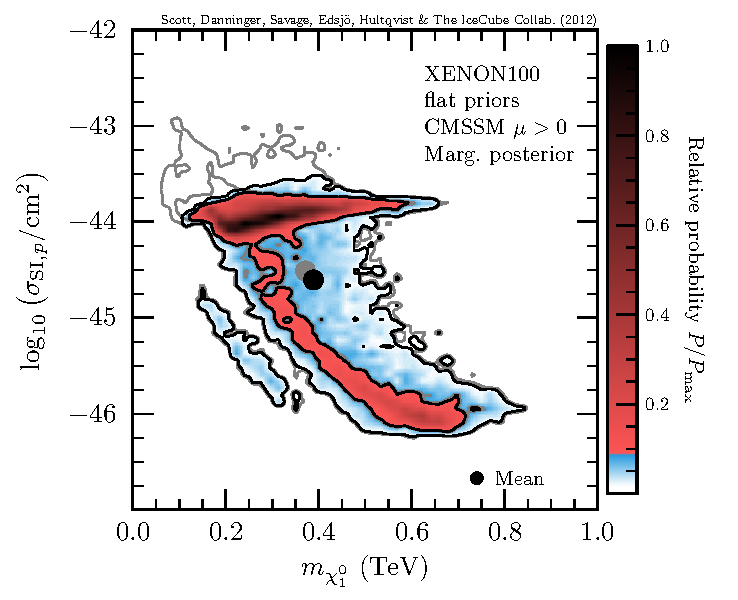
\includegraphics[height=0.95\linewidth, trim = 0 0 8 0, clip = true]{marg2D_2_2}}%
\only<4>{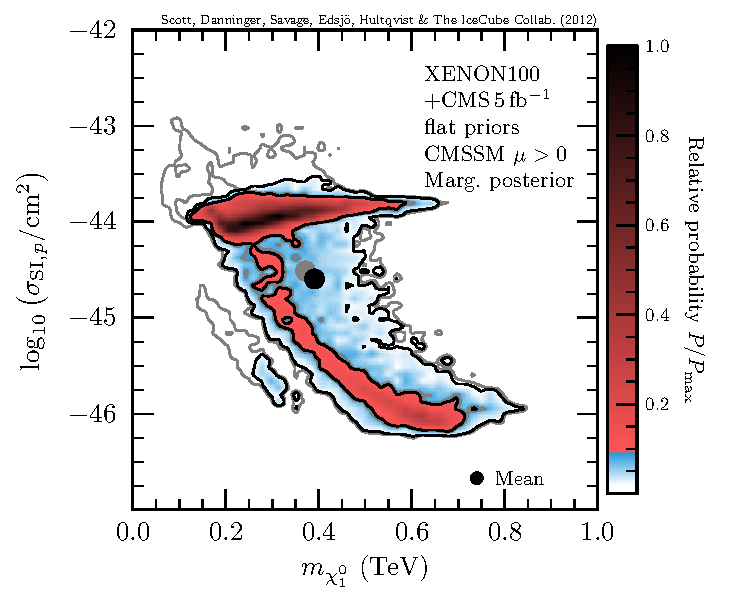
\includegraphics[height=0.95\linewidth, trim = 0 0 8 0, clip = true]{marg2D_3_2}}%
\only<5->{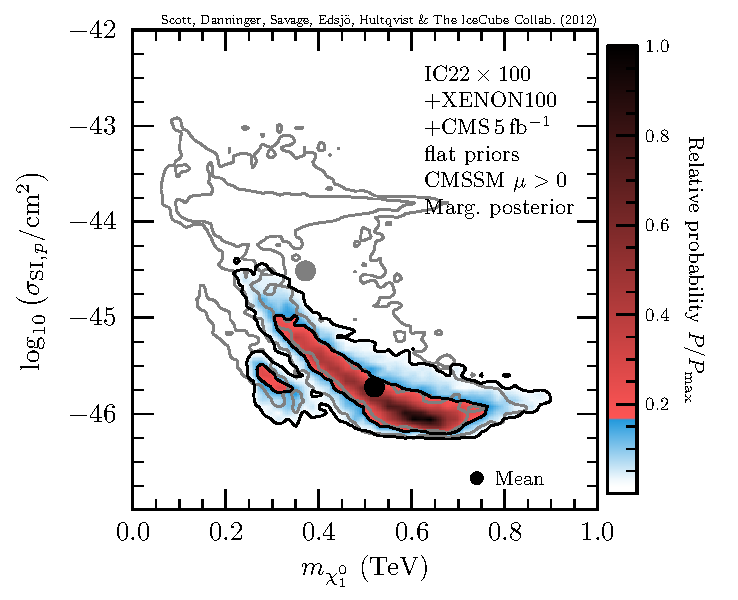
\includegraphics[height=0.95\linewidth, trim = 0 0 8 0, clip = true]{marg2D_4_2}}

\end{columns}\vspace{5mm}

\visible<6->{\alert{``Astroparticle road to new physics''} = finding/constraining new physics with astro AND particle data as co-navigators\vspace{3mm}}

\visible<7->{This example is a gross simplification -- the devil is in the detail.\vspace{3mm}}

\visible<7->{Many talk about complementarity, far fewer walk the walk quantitatively $\rightarrow$ global BSM fits}

\end{frame}



\begin{frame}
\frametitle{Global fits in the current era}

Lots of data flowing from LHC, direct and indirect dark matter detection experiments

$\rightarrow$ new ``Implications of $\langle data\ X\rangle$ for supersymmetry'' fit update every few months\vspace{5mm}

Issues with current global fit codes:
\begin{itemize}
\item Strongly wedded to a few theories (e.g. constrained minimal SUSY Standard Model)
\item Strongly wedded to a few theory calculators
\item All datasets and observables basically hardcoded
\item Rough or non-existent treatment of most experiments (astroparticle + collider especially)
\item Sub-optimal statistical methods / search algorithms
\item $\implies$ \textit{already hitting the wall on theories, data \& computational methods}
\end{itemize}

\end{frame}



\begin{frame}
\frametitle{\textbf{GAMBIT}: a \textit{second-generation} global fit code}

GAMBIT: \alert{G}lobal \alert{A}nd \alert{M}odular \alert{B}SM \alert{I}nference \alert{T}ool
\vspace{5mm}

Overriding principles of GAMBIT: flexibility and modularity
\begin{itemize}
\item General enough to allow fast definition of new datasets and theoretical models
\item Plug and play scanning, physics and likelihood packages
\item Extensive model database -- not just small modifications to constrained MSSM (NUHM, etc), and not just SUSY!
\item Extensive observable/data libraries (likelihood modules)
\item Many statistical options -- Bayesian/frequentist, likelihood definitions, scanning algorithms
\item A smart and \textit{fast} LHC likelihood calculator
\item Massively parallel
\item Full open-source code release
\end{itemize}

\end{frame}


\begin{frame}
\frametitle{The GAMBIT Collaboration \only<2->{\alert{-- the future}}}

\only<1>{23}\only<2->{\alert{28}} Members, \only<1>{12}\only<2->{\alert{14}} Institutes\only<3>{, \cblue{6 UK members}} \\
\only<1>{8}\only<2->{\alert{10}} Experiments, 3 major theory codes \vspace{3mm}

\begin{tabular}{l l}
\textbf{Fermi-LAT} & \small \alert<1>{\cbluewhen{P.\ Scott}{<3>}}, J. Conrad, J. Edsj\"o, G. Martinez\\
\textbf{IceCube} & \small \alert<1>{\cbluewhen{P.\ Scott}{<3>}}, J.\ Edsj\"o, C.\ Savage\\
\textbf{ATLAS} & \small \cbluewhen{A.\ Buckley}{<3>}, C.\ Clement, P.\ Jackson, A.\ Saavedra, M.\ White\\
\textbf{CMS} & \small C.\ Rogan, \visible<2->{\alert<2>{\cbluewhen{+2 (Imperial)}{<3>}}}\\
\textbf{HESS} & \small J.\ Conrad, H.\ Dickinson \\
\textbf{AMS-02} & \small A.\ Putze\\
\textbf{CTA} & \small T.\ Bringmann, J.\ Conrad, H.\ Dickinson\\
\textbf{DARWIN} & \small J.\ Conrad\\
\textbf{Theory} & \small \alert<1>{\cbluewhen{P.\ Scott}{<3>}}, C. Bal\'azs, T.\ Bringmann, L.-A.\ Dal, J.\ Edsj\"o, \\
                & \small B.\ Farmer, A.\ Krislock, A.\ Kvellestad, N.\ Mahmoudi, \\
                & \small A.\ Raklev, C.\ Savage, C.\ Weniger \\
\visible<2->{\alert{\textbf{LUX/LZ}}  & \small \alert<2>{\cbluewhen{+1 (Imperial)}{<3>}}\\
\alert{\textbf{LHCb}}    & \small \alert{2 members approached} \visible<3>{\cblue{(one UK)}} 
}
\end{tabular}

\end{frame}


\begin{frame}
\frametitle{Plans -- GAMBIT and the Rutherford Fellowship}

The point is not just to write code -- but to \textbf{*use*} it\ldots
\begin{itemize}
\item Aiming for first comprehensive 25-parameter MSSM global analysis 
\item Extensive SUSY-breaking model comparison
\item Global fits to many non-SUSY models (2 Higgs Doublet, extra dimensions, isospin-violating dark matter, etc)
\item Model comparison of different BSM scenarios
\item Each physics module, + scanner module, will have dedicated paper and code release
\item GAMBIT code will become the go-to package, and GAMBIT papers the go-to results, for combined interpretation of BSM physics searches in the future
\end{itemize}

\end{frame}


\end{document}

